\documentclass[aspectratio=169,11pt]{beamer}

% =========================================================
% Packages
% =========================================================
\usepackage{amsmath,amssymb,mathtools,bm}
\usepackage{booktabs}
\usepackage{array}
\usepackage{ragged2e}
\usepackage{microtype}
\usepackage{graphicx}
\usepackage{xcolor}

% =========================================================
% Theme
% =========================================================
\usetheme{Boadilla}
\usecolortheme{default}
\setbeamertemplate{navigation symbols}{}
\setbeamertemplate{footline}[frame number]

\definecolor{DeepBlue}{RGB}{28,66,120}
\definecolor{DarkGray}{RGB}{55,55,55}
\definecolor{SoftGray}{RGB}{242,242,242}
\definecolor{DarkRed}{RGB}{155,45,45}
\definecolor{DarkGreen}{RGB}{35,110,75}

\setbeamercolor{structure}{fg=DeepBlue}
\setbeamercolor{frametitle}{fg=DeepBlue}
\setbeamercolor{title}{fg=DeepBlue}
\setbeamercolor{block title}{bg=DeepBlue!12,fg=DeepBlue}
\setbeamercolor{block body}{bg=DeepBlue!3,fg=black}
\setbeamercolor{alerted text}{fg=DarkRed}

% =========================================================
% Layout tuning (compact vertical rhythm)
% =========================================================
\setbeamersize{text margin left=1.1em,text margin right=1.1em}

% Many slides contain several display equations; the default
% display skips are the single largest source of overfull frames.
\AtBeginDocument{%
  \setlength{\abovedisplayskip}{3.5pt plus 2pt minus 1.5pt}%
  \setlength{\belowdisplayskip}{3.5pt plus 2pt minus 1.5pt}%
  \setlength{\abovedisplayshortskip}{1.5pt plus 1pt minus 1pt}%
  \setlength{\belowdisplayshortskip}{2.5pt plus 1pt minus 1pt}%
  \setlength{\jot}{2pt}%
}

% Tighter blocks: trim the space around the box, not its inner padding
\addtobeamertemplate{block begin}{\vspace{-0.45em}}{}
\addtobeamertemplate{block end}{}{\vspace{-0.35em}}
\addtobeamertemplate{block alerted begin}{\vspace{-0.45em}}{}
\addtobeamertemplate{block alerted end}{}{\vspace{-0.35em}}

% Tighter lists
\setlength{\leftmargini}{1.5em}
\setbeamertemplate{itemize/enumerate body begin}{\vspace{-0.2em}}
\setbeamertemplate{itemize/enumerate body end}{\vspace{-0.2em}}

% Slightly tighter frame titles
\setbeamerfont{frametitle}{size=\large,series=\bfseries}

% Ragged-right table columns; narrow columns look much calmer when
% they are not hyphenated on nearly every line.
\newcommand{\NoHyph}{\hyphenpenalty=10000\exhyphenpenalty=10000\relax}
\newcolumntype{L}[1]{>{\RaggedRight\NoHyph\arraybackslash}p{#1}}
\newcolumntype{B}[1]{>{\RaggedRight\NoHyph\bfseries\arraybackslash}p{#1}}

% =========================================================
% Commands
% =========================================================
\newcommand{\E}{\mathbb{E}}
\newcommand{\Pp}{\mathbb{P}}
\newcommand{\ind}{\mathbf{1}}
\newcommand{\ATE}{\mathrm{ATE}}
\newcommand{\ATT}{\mathrm{ATT}}

\newcommand{\Question}{\textcolor{DarkRed}{\textbf{Question}}}
\newcommand{\Spec}{\textcolor{DeepBlue}{\textbf{Specification \& Estimand}}}
\newcommand{\Ident}{\textcolor{DarkGreen}{\textbf{Identification}}}
\newcommand{\Est}{\textcolor{violet}{\textbf{Estimation}}}
\newcommand{\Infer}{\textcolor{orange!80!black}{\textbf{Inference}}}


% Recitation-specific additions
\usepackage{pgfplots}
\pgfplotsset{compat=1.16}
\usepackage{listings}
\lstdefinestyle{stata}{
  basicstyle=\ttfamily\scriptsize,
  commentstyle=\color{DarkGreen},
  keywordstyle=\color{DeepBlue}\bfseries,
  morekeywords={ivprobit,probit,regress,predict,margins,eprobit,heckman,
    generate,bcuse},
  morecomment=[l]{//},
  columns=fullflexible,
  keepspaces=true,
  backgroundcolor=\color{SoftGray},
  frame=none,
  xleftmargin=0.4em,
  aboveskip=0.3em,
  belowskip=0.3em
}

\newcommand{\Part}[1]{\textcolor{DarkRed}{\textbf{(#1)}}}
\newcommand{\Mills}{\lambda}

% =========================================================
% Title
% =========================================================
\title{Mostly Harmless Econometrics}
\subtitle{
\textbf{Session 1.1: Recitation}
\\[0.55em]
Endogenous Regressors in Binary Choice
$\;\&\;$
the Heckman Sample Selection Model
}
\author{Kaiwen Luo}
\institute{Washington University in St.Louis}
\date{\today}

\begin{document}

% =========================================================
\begin{frame}
    \titlepage
\end{frame}

% =========================================================
\begin{frame}{Today: two problems, one structure}

Both problems are about \textbf{female labor supply}, and both share the
same skeleton:
\begin{center}
\textit{two equations} $+$ \textit{jointly normal errors} $+$
\textit{one outcome only partially observed}.
\end{center}

We answer the same four questions for each, and map them onto the
workflow from Session 1:

\vspace{0.05em}

\small
\begin{tabular}{B{0.30\textwidth} L{0.24\textwidth} L{0.36\textwidth}}
\toprule
Sub-question & Workflow step & What we must show\\
\midrule
\Part{1} Propose an estimator & \Est &
  Two-step control function and full MLE\\[0.1em]
\Part{2} Assumption for identification & \Ident &
  Exclusion restriction $+$ relevance\\[0.1em]
\Part{3} Same regressors in both equations & \Ident{} (failure) &
  What survives: reduced-form parameters\\[0.1em]
\Part{4} Stata command & \Est{} \& \Infer &
  Implementation and correct standard errors\\
\bottomrule
\end{tabular}

\vspace{0.4em}

\begin{alertblock}{Reading order}
The problem asks \Part{1} before \Part{2}. Logically, \Part{2} comes first:
an estimator is only meaningful once we know what it converges to.
\end{alertblock}

\end{frame}

% =========================================================
\section{Part I: An Endogenous Regressor in a Probit}

\begin{frame}{Problem 1: the setup}

Female labor market participation with endogenous non-labor income:
\begin{align*}
y &= \ind\{x_y'\beta + w\gamma + \varepsilon > 0\}
  &&\text{(participation)}\\
w &= x_w'\eta + \sigma_w v
  &&\text{(non-labor income)}
\end{align*}
\[
(\varepsilon, v)\mid x_y, x_w \sim N\!\left(\bm 0,\;
\begin{pmatrix} 1 & \rho\\ \rho & 1\end{pmatrix}\right).
\qquad
\text{\textcolor{DarkGray}{\footnotesize (the problem's $u$ is $\varepsilon$)}}
\]

\begin{columns}[T]
\column{0.48\textwidth}
\begin{block}{Observed}
$y\in\{0,1\}$, \; $w\in\mathbb R$, \; $x_y$, \; $x_w$.
\end{block}
\column{0.48\textwidth}
\begin{block}{Unknown}
$\beta,\;\gamma,\;\eta,\;\sigma_w,\;\rho$.
\end{block}
\end{columns}

\vspace{0.3em}

\begin{enumerate}\small
  \item[\Part{1}] Propose a method to estimate this model.
  \item[\Part{2}] Which assumption identifies $\gamma$? Show how.
  \item[\Part{3}] If $x_y=x_w$, which reduced-form parameters involving $\gamma$ are identified?
  \item[\Part{4}] Which Stata command estimates this model?
\end{enumerate}

\end{frame}

% =========================================================
\begin{frame}{Before estimating: read the specification}

\textbf{What is $\gamma$?} The effect of non-labor income on the latent
propensity to work. Theory (income effect $\Rightarrow$ higher reservation
wage) suggests $\gamma<0$.

\pause

\vspace{0.3em}

\textbf{Why is $w$ endogenous?} Unobserved household wealth, a spouse's
earnings potential, or a taste for home production shift \emph{both}
$w$ and the decision to work:
\[
\operatorname{Cov}(\varepsilon,\,w\mid x_y,x_w)
=\operatorname{Cov}(\varepsilon,\,\sigma_w v)=\rho\,\sigma_w\neq 0 .
\]

\pause

\textbf{Normalizations.} $y^*$ is never observed, so its scale is not
identified: $\operatorname{Var}(\varepsilon)=1$. The scale of $w$
\emph{is} observed and is carried by $\sigma_w$, so
$\operatorname{Var}(v)=1$ is a relabeling, not a restriction.

\pause

\vspace{0.3em}

\begin{alertblock}{Why the naive probit fails}
A probit of $y$ on $(x_y,w)$ assumes $\varepsilon\perp w$. Here
$\E[\varepsilon\mid w,x]=\rho v\neq 0$, so the coefficient on $w$ mixes
the causal effect $\gamma$ with the selection term $\rho/\sigma_w$.
\end{alertblock}

\end{frame}

% =========================================================
\begin{frame}{The key trick: decompose $\varepsilon$ given $v$}

Joint normality gives a linear projection with an independent remainder:
\[
\varepsilon = \rho\, v + e,
\qquad
e \sim N(0,\,1-\rho^2),
\qquad
e \perp (v, x_y, x_w).
\]

\pause

Given $(x_y,x_w,w)$, the residual $v=(w-x_w'\eta)/\sigma_w$ is known.
Hence
\[
\Pp(y=1\mid x_y,x_w,w)
=\Pp\!\left(e > -x_y'\beta - w\gamma - \rho v\right)
\]
\[
\boxed{
\Pp(y=1\mid x_y,x_w,w)
=\Phi\!\left(
\frac{x_y'\beta + w\gamma + \rho\,v}{\sqrt{1-\rho^2}}
\right)
}
\]

\pause

\begin{block}{Interpretation: a control function}
Once we condition on $v$, the part of $\varepsilon$ that is correlated with
$w$ is held fixed. What remains, $e$, is independent of $w$:
$v$ ``controls for'' the source of endogeneity.
\end{block}

\end{frame}

% =========================================================
\subsection{(1) Estimation}

\begin{frame}{\Part{1} Method A: two-step control function}

\textcolor{DarkGray}{Rivers and Vuong (1988); Smith and Blundell (1986) for the Tobit.}

\vspace{0.3em}

\textbf{Step 1.} OLS of $w$ on $x_w$:
\[
\hat\eta,\qquad
\hat\sigma_w^2=\tfrac1n\textstyle\sum_i (w_i-x_{w,i}'\hat\eta)^2,\qquad
\hat v_i = (w_i - x_{w,i}'\hat\eta)/\hat\sigma_w .
\]

\textbf{Step 2.} Probit of $y$ on $(x_y,\,w,\,\hat v)$:
\[
\Pp(y=1\mid x_y,w,\hat v)
=\Phi\!\left(x_y'\beta_\rho + w\gamma_\rho + \hat v\,\theta_\rho\right),
\qquad
(\beta_\rho,\gamma_\rho,\theta_\rho)=\frac{(\beta,\,\gamma,\,\rho)}{\sqrt{1-\rho^2}} .
\]

\pause

\textbf{Step 3.} Undo the scaling. Since $1+\theta_\rho^2 = 1/(1-\rho^2)$,
\[
\hat\rho=\frac{\hat\theta_\rho}{\sqrt{1+\hat\theta_\rho^2}},
\qquad
\hat\gamma=\frac{\hat\gamma_\rho}{\sqrt{1+\hat\theta_\rho^2}},
\qquad
\hat\beta=\frac{\hat\beta_\rho}{\sqrt{1+\hat\theta_\rho^2}} .
\]

\pause

\begin{block}{Why it works}
Step 1 makes the control $v$ observable; Step 2 is then an ordinary probit
whose error $e/\sqrt{1-\rho^2}$ is standard normal and independent of all regressors.
\end{block}

\end{frame}

% =========================================================
\begin{frame}{\Part{1} Inference for the two-step estimator}

\begin{block}{Generated regressor}
$\hat v_i$ is estimated, not observed. The usual probit standard errors
from Step 2 ignore the sampling error in $(\hat\eta,\hat\sigma_w)$ and are
\textbf{too small}.
Fix: Murphy--Topel correction, or bootstrap \emph{both} steps together.
\end{block}

\pause

\begin{block}{A free test of exogeneity}
Under $H_0:\rho=0$ we have $\theta_\rho=0$, so the first-step error
does not affect Step 2. The \emph{usual} $t$-statistic on $\hat v$ is a
valid test of $H_0:\; w$ is exogenous.
\end{block}

\pause

\begin{alertblock}{Do not ``plug in'' $\hat w$}
Replacing $w$ by $\hat w = x_w'\hat\eta$ in a probit (a ``forbidden
regression'') leaves the composite error $\varepsilon+\gamma\sigma_w v$,
with variance $1+2\rho\gamma\sigma_w+\gamma^2\sigma_w^2$ that depends on
$\gamma$. It recovers $(\beta,\gamma)$ only up to this unknown scale, relies on
exact normality, and does not generalize to other nonlinear models.
\end{alertblock}

\end{frame}

% =========================================================
\begin{frame}{\Part{1} Method B: full maximum likelihood}

Factor the joint density of what we observe:
\[
f(y,w\mid x)
=\underbrace{\Pp(y\mid w,x)}_{\text{probit with control}}
\cdot
\underbrace{f(w\mid x)}_{N(x_w'\eta,\;\sigma_w^2)} .
\]

\pause

With $v_i=(w_i-x_{w,i}'\eta)/\sigma_w$ and
$\displaystyle m_i=\frac{x_{y,i}'\beta + w_i\gamma + \rho\,v_i}{\sqrt{1-\rho^2}}$,
the log-likelihood is
\[
\boxed{
\ell(\beta,\gamma,\eta,\sigma_w,\rho)
=\sum_i\Big\{
y_i\log\Phi(m_i)+(1-y_i)\log\big[1-\Phi(m_i)\big]
+\log\phi(v_i)-\log\sigma_w
\Big\}}
\]

\pause

\begin{itemize}
  \item Efficient under the model; standard errors come directly from the Hessian.
  \item In practice, optimize over $\operatorname{atanh}\rho$ and $\log\sigma_w$ so the parameter space is unrestricted.
  \item The two-step estimates are good starting values.
\end{itemize}

\end{frame}

% =========================================================
\begin{frame}{\Part{1} Coefficients are not the end: what is the estimand?}

The model gives $\gamma$ only \emph{in units of} $\operatorname{sd}(\varepsilon)$.
A policy question is usually about probabilities.

\vspace{0.3em}

\textbf{Average structural function} (Blundell and Powell, 2004):
\[
\operatorname{ASF}(x_y,w)=\E_\varepsilon\big[\ind\{x_y'\beta+w\gamma+\varepsilon>0\}\big]
=\Phi(x_y'\beta+w\gamma).
\]

\pause

With the two-step estimates, average over the control function instead:
\[
\widehat{\operatorname{ASF}}(x_y,w)
=\frac1n\sum_{i=1}^n
\Phi\big(x_y'\hat\beta_\rho+w\hat\gamma_\rho+\hat v_i\hat\theta_\rho\big)
\;\xrightarrow{p}\;
\Phi(x_y'\beta+w\gamma),
\]
because $\rho v+e\sim N(0,1)$.

\pause

\begin{block}{Average partial effect of non-labor income}
\[
\operatorname{APE}_w=\E\!\left[\gamma\,\phi(x_y'\beta+w\gamma)\right]
\]
This is the object to compare with a linear probability model estimated by 2SLS.
\end{block}

\end{frame}

% =========================================================
\subsection{(2) Identification}

\begin{frame}{\Part{2} The assumption: an exclusion restriction}

Split the first-stage index into variables that do and do not enter $y$:
\[
x_w'\eta = x_y'\pi_1 + z'\pi_2,
\qquad z = \text{variables in } x_w \text{ excluded from } x_y .
\]

\begin{block}{Assumption (exclusion $+$ relevance)}
There is at least one variable $z$ that
\begin{enumerate}
  \item does not enter the participation equation \hfill (exclusion)
  \item shifts non-labor income: $\pi_2\neq 0$ \hfill (relevance)
  \item and $\E[(x_y, z)(x_y, z)']$ has full rank \hfill (no redundancy)
\end{enumerate}
\end{block}

\pause

\textbf{Example:} husband's education shifts household non-labor income,
but (arguably) not the wife's own taste for work.

\vspace{0.3em}

\begin{alertblock}{Exactly as in linear IV}
Normality buys us the shape of $\Pp(y=1\mid\cdot)$. It does \emph{not}
replace the instrument.
\end{alertblock}

\end{frame}

% =========================================================
\begin{frame}{\Part{2} Showing that $\gamma$ is identified}

\textbf{Step 1: the first stage.}
$\E[w\mid x]=x_w'\eta$ and $\operatorname{Var}(w\mid x)=\sigma_w^2$ identify
$(\eta,\sigma_w)$. Therefore $v=(w-x_w'\eta)/\sigma_w$ is a known function
of observables.

\pause

\textbf{Step 2: invert the probit.} Since $\Phi$ is strictly increasing,
\[
\Phi^{-1}\!\big(\Pp(y=1\mid x,w)\big)
= x_y'\beta_\rho + w\gamma_\rho + v\,\theta_\rho .
\]
The left side is a known function of the data. The coefficients are
identified iff $(x_y,\,w,\,v)$ are not perfectly collinear.

\pause

\textbf{Step 3: rule out collinearity.}
\[
w = x_y'\pi_1 + z'\pi_2 + \sigma_w v .
\]
$w$ is a linear combination of $(x_y,v)$ \;$\Longleftrightarrow$\; $z'\pi_2\equiv0$.
The exclusion restriction with $\pi_2\neq0$ rules this out.

\pause

\textbf{Step 4: undo the scaling.}
$\rho=\theta_\rho/\sqrt{1+\theta_\rho^2}$ and
$\gamma=\gamma_\rho/\sqrt{1+\theta_\rho^2}$. \hfill $\blacksquare$

\end{frame}

% =========================================================
\begin{frame}{\Part{2} The intuition}

Think of $v$ as a woman's unobserved ``type''.

\vspace{0.3em}

\begin{columns}[T]
\column{0.48\textwidth}
\begin{block}{With an instrument}
Fix $x_y$ and $v$. Varying $z$ still moves $w$.

Any resulting change in $\Pp(y=1)$ must come from $\gamma$, since the
type is held fixed.
\end{block}

\column{0.48\textwidth}
\begin{block}{Without an instrument}
Fix $x_y$ and $v$. Then $w$ is fixed too.

Every movement in $w$ comes with a movement in $v$, so $\gamma$ cannot be
separated from $\rho$.
\end{block}
\end{columns}

\vspace{0.6em}

\begin{center}
\boxed{
\text{Identification} = \text{variation in } w
\text{ that is not variation in the unobservables}
}
\end{center}

\vspace{0.4em}

This is the logic of the first stage in 2SLS. Part \Part{3} makes the
failure case concrete.

\end{frame}

% =========================================================
\subsection{(3) No exclusion restriction}

\begin{frame}{\Part{3} When $x_y=x_w=x$: substitute out $v$}

Now $v=(w-x'\eta)/\sigma_w$, and the probit index becomes
\[
\frac{x'\beta + w\gamma + \rho\,(w-x'\eta)/\sigma_w}{\sqrt{1-\rho^2}}
= x'\underbrace{\frac{\beta-\rho\,\eta/\sigma_w}{\sqrt{1-\rho^2}}}_{\equiv\,a}
+ w\,\underbrace{\frac{\gamma+\rho/\sigma_w}{\sqrt{1-\rho^2}}}_{\equiv\,b} .
\]

\pause

\begin{block}{What the data identify}
From $f(w\mid x)$: \;$\eta,\ \sigma_w$.
\qquad
From $\Pp(y=1\mid x,w)=\Phi(x'a+wb)$: \;$a,\ b$.

These four objects pin down the entire distribution of $(y,w)\mid x$.
\end{block}

\pause

\begin{block}{Equivalently: the reduced form for $y$ alone}
Substituting $w$ into the $y$ equation,
$y=\ind\{x'(\beta+\gamma\eta)+\varepsilon+\gamma\sigma_w v>0\}$, so
\[
\Pp(y=1\mid x)=\Phi(x'\pi),\qquad
\pi=\frac{\beta+\gamma\eta}{\omega},\qquad
\omega^2=1+2\rho\gamma\sigma_w+\gamma^2\sigma_w^2 .
\]
One can check that $\pi=(a+b\eta)/\sqrt{1+b^2\sigma_w^2}$: nothing new.
\end{block}

\end{frame}

% =========================================================
\begin{frame}{\Part{3} Why $\gamma$ itself is lost}

\textbf{Counting.} Unknowns $(\beta,\gamma,\rho)$: $\;k+2$.
Identified $(a,b)$: $\;k+1$. One equation short.

\pause

\textbf{Observational equivalence.} Pick any $\tilde\rho\in(-1,1)$ and set
\[
\tilde\gamma=b\sqrt{1-\tilde\rho^2}-\tilde\rho/\sigma_w,
\qquad
\tilde\beta=a\sqrt{1-\tilde\rho^2}+\tilde\rho\,\eta/\sigma_w .
\]
Then $(\tilde\beta,\tilde\gamma,\tilde\rho)$ produces the same $(a,b)$, hence the same data.

\pause

\begin{block}{What the identified parameter means}
\[
b\sqrt{1-\rho^2}
=\gamma+\frac{\rho}{\sigma_w}
=\underbrace{\gamma}_{\text{causal}}
+\underbrace{\frac{\operatorname{Cov}(\varepsilon,w\mid x)}{\operatorname{Var}(w\mid x)}}_{\text{selection on unobservables}}
\]
The familiar omitted-variable-bias formula, inside a probit.
\end{block}

\pause

\begin{alertblock}{Normality does not rescue us here}
The control $\rho v$ enters the index \emph{linearly}, so it is exactly
collinear with $(x,w)$. Only outside information on $\rho$ (e.g.\
$\rho=0$, or its sign) turns $b$ into a statement about $\gamma$.
\end{alertblock}

\end{frame}

% =========================================================
\subsection{(4) Stata}

\begin{frame}[fragile]{\Part{4} Stata}

Wooldridge's \texttt{mroz} data: \texttt{inlf} $=y$, \texttt{nwifeinc} $=w$, \texttt{huseduc} $=z$.

\begin{lstlisting}[style=stata]
bcuse mroz, clear                         // ssc install bcuse

// (a) Full MLE (default)
ivprobit inlf educ exper expersq age kidslt6 kidsge6 (nwifeinc = huseduc)
margins, dydx(nwifeinc) predict(pr)       // APE from the structural probability

// (b) Two-step estimator (Newey 1987), corrected standard errors
ivprobit inlf educ exper expersq age kidslt6 kidsge6 (nwifeinc = huseduc), twostep

// (c) Control function by hand: point estimates only, bootstrap the SEs
regress nwifeinc educ exper expersq age kidslt6 kidsge6 huseduc
predict vhat, residuals
probit  inlf educ exper expersq age kidslt6 kidsge6 nwifeinc vhat

// (d) Extended regression models (Stata 15+)
eprobit inlf educ exper expersq age kidslt6 kidsge6, ///
        endogenous(nwifeinc = educ exper expersq age kidslt6 kidsge6 huseduc)
\end{lstlisting}

\vspace{-0.2em}
\footnotesize
\begin{itemize}
  \item \texttt{ivprobit} reports a Wald test of exogeneity ($H_0:\rho=0$);
        in (c), the $t$-test on \texttt{vhat} is the same idea.
  \item Stata's first stage regresses $w$ on \emph{all} exogenous variables, $x_y\cup x_w$.
\end{itemize}

\end{frame}

% =========================================================
\section{Part II: The Heckman Sample Selection Model}

\begin{frame}{Problem 2: the setup}

\textcolor{DarkGray}{Gronau (1974); Heckman (1979).}
We want the \textbf{wage offer} equation for \emph{all} women, but wages
are observed only for those who work:
\begin{align*}
y &= x'\beta + u_1
  &&\text{(log wage offer, observed iff } d=1)\\
d &= \ind\{z'\delta + u_2 > 0\}
  &&\text{(participation)}
\end{align*}
\[
(u_1, u_2)\mid x,z \sim N\!\left(\bm 0,\;
\begin{pmatrix} \sigma^2 & \rho\sigma\\ \rho\sigma & 1\end{pmatrix}\right).
\]

\begin{columns}[T]
\column{0.48\textwidth}
\begin{block}{Observed}
$d$ and $(x,z)$ for everyone; \; $y$ only if $d=1$.
\end{block}
\column{0.48\textwidth}
\begin{block}{Unknown}
$\beta,\;\delta,\;\sigma,\;\rho$.
\end{block}
\end{columns}

\vspace{0.3em}

\begin{enumerate}\small
  \item[\Part{1}] Propose a method to estimate this model.
  \item[\Part{2}] Which assumption identifies $\beta$? Show how.
  \item[\Part{3}] If $x=z$, what can still be identified?
  \item[\Part{4}] Which Stata command estimates this model?
\end{enumerate}

\end{frame}

% =========================================================
\begin{frame}{Before estimating: read the specification}

\textbf{What is $\beta$?} E.g.\ the return to education in the
\emph{offered} wage, for the whole population of women.
It is \textbf{not} the slope of observed wages among workers.

\pause

\vspace{0.3em}

\textbf{Why is OLS on workers biased?} Women who work may be those with
unusually good wage offers:
\[
\E[y\mid x,z,d=1]=x'\beta+\E[u_1\mid u_2>-z'\delta]\neq x'\beta
\quad\text{when }\rho\neq 0 .
\]
The bias term varies with $z$, which overlaps with $x$, so the slopes are
biased, not just the intercept.

\pause

\textbf{Normalizations.} $d^*$ is latent: $\operatorname{Var}(u_2)=1$.
$y$ is observed in levels, so $\sigma$ is a free parameter.

\vspace{0.3em}

\begin{alertblock}{Compare with Part I}
Part I: a \emph{regressor} is endogenous.
Part II: the \emph{sample} is endogenous.
Once written down, both are omitted-variable problems.
\end{alertblock}

\end{frame}

% =========================================================
\begin{frame}{The key trick again: decompose $u_1$ given $u_2$}

Joint normality:
\[
u_1=\rho\sigma\,u_2 + e,\qquad e\sim N\big(0,\sigma^2(1-\rho^2)\big),
\qquad e\perp (u_2,x,z).
\]

\pause

Truncated normal mean: for $c=z'\delta$,
\[
\E[u_2\mid u_2>-c]=\frac{\phi(c)}{\Phi(c)}\equiv\Mills(c)
\qquad\text{(inverse Mills ratio)}.
\]

\pause

Therefore
\[
\boxed{
\E[y\mid x,z,d=1]
= x'\beta + \underbrace{\rho\sigma}_{\equiv\,\theta}\,\Mills(z'\delta)
}
\]

\pause

\begin{block}{Interpretation: a control function}
Selection bias is an \textbf{omitted variable}, $\Mills(z'\delta)$.
Part I controlled for $v$, the residual of a \emph{continuous} first stage;
here we control for $\Mills$, the generalized residual of a
\emph{binary} first stage.
\end{block}

\end{frame}

% =========================================================
\subsection{(1) Estimation}

\begin{frame}{\Part{1} Method A: Heckman's two-step (``Heckit'')}

\textbf{Step 1.} Probit of $d$ on $z$, using the full sample:
\[
\hat\delta,\qquad \hat\Mills_i=\frac{\phi(z_i'\hat\delta)}{\Phi(z_i'\hat\delta)} .
\]

\textbf{Step 2.} OLS of $y$ on $(x,\;\hat\Mills)$, using workers only ($d_i=1$):
\[
y_i = x_i'\beta + \theta\,\hat\Mills_i + \text{error}_i .
\]

\pause

\begin{block}{Inference}
\begin{itemize}
  \item The error is \textbf{heteroskedastic}:
  $\operatorname{Var}(y\mid x,z,d=1)=\sigma^2-\theta^2\Mills(c)\big[\Mills(c)+c\big]$, $c=z'\delta$.
  \item $\hat\Mills$ is a \textbf{generated regressor}: OLS standard errors are wrong.
  \item Free test: under $H_0:\rho=0$, the usual $t$-test on $\hat\Mills$
        is valid. \hfill (Same as $\hat v$ in Part I.)
\end{itemize}
\end{block}

\pause

\textbf{Recover $\sigma,\rho$:}
$\hat\sigma^2=\frac{1}{n_1}\sum_{d_i=1}\big[\hat e_i^2+\hat\theta^2\hat\Mills_i(\hat\Mills_i+z_i'\hat\delta)\big]$,
\;$\hat\rho=\hat\theta/\hat\sigma$.

\end{frame}

% =========================================================
\begin{frame}{\Part{1} Method B: full maximum likelihood}

The two kinds of observations contribute differently:
\[
d_i=0:\quad \Pp(d=0\mid z)=1-\Phi(z_i'\delta)
\]
\[
d_i=1:\quad f(y\mid x)\cdot\Pp(d=1\mid y,x,z)
=\frac1\sigma\phi\!\left(\frac{y_i-x_i'\beta}{\sigma}\right)
\Phi\!\left(\frac{z_i'\delta+\frac{\rho}{\sigma}(y_i-x_i'\beta)}{\sqrt{1-\rho^2}}\right)
\]

\pause

\[
\boxed{
\ell=\sum_{d_i=0}\log\big[1-\Phi(z_i'\delta)\big]
+\sum_{d_i=1}\left\{
\log\Phi\!\left(\frac{z_i'\delta+\frac{\rho}{\sigma}(y_i-x_i'\beta)}{\sqrt{1-\rho^2}}\right)
-\log\sigma+\log\phi\!\left(\frac{y_i-x_i'\beta}{\sigma}\right)
\right\}}
\]

\pause

\begin{columns}[T]
\column{0.48\textwidth}
\begin{block}{MLE}
Efficient if the model is right; joint normality is used everywhere.
\end{block}
\column{0.48\textwidth}
\begin{block}{Two-step}
Needs only normal $u_2$ and linear $\E[u_1\mid u_2]$. Simpler and more
robust, but less efficient.
\end{block}
\end{columns}

\vspace{0.3em}

Parallel with Part I: the $d=1$ term is a \emph{probit with a
control} times a \emph{normal density}.

\end{frame}

% =========================================================
\subsection{(2) Identification}

\begin{frame}{\Part{2} The assumption: an exclusion restriction}

\begin{block}{Assumption (exclusion $+$ relevance)}
$z$ contains at least one variable that
\begin{enumerate}
  \item does not affect the wage offer: it is excluded from $x$ \hfill (exclusion)
  \item shifts participation: its coefficient in $\delta$ is nonzero \hfill (relevance)
\end{enumerate}
\end{block}

\pause

\textbf{Classic choices:} number of young children, and
\textbf{non-labor income}.
Non-labor income raises the reservation wage, so it shifts
participation; an employer's wage offer does not depend on it.

\pause

\vspace{0.3em}

\begin{alertblock}{Notice the reversal}
In Part I, non-labor income was the \emph{endogenous regressor} that
needed an instrument. In Part II, the same variable \emph{is} the
instrument.

Exogeneity is a property of a variable \emph{in an equation}, relative to
a question, not of the variable itself.
\end{alertblock}

\end{frame}

% =========================================================
\begin{frame}{\Part{2} Showing that $\beta$ is identified}

\textbf{Step 1: the selection equation.}
$\Pp(d=1\mid z)=\Phi(z'\delta)$ identifies $\delta$, using all observations.
Hence $\Mills(z'\delta)$ is a known function of observables.

\pause

\textbf{Step 2: the selected sample.}
$\E[y\mid x,z,d=1]=x'\beta+\theta\,\Mills(z'\delta)$, so
$(\beta,\theta)$ are identified iff $\E\big[(x,\Mills)(x,\Mills)'\mid d=1\big]$
has full rank.

\pause

\textbf{Step 3: rule out collinearity.}
With an excluded $z_k$ and $\delta_k\neq0$, $\Mills(z'\delta)$ moves while
$x$ is held fixed, so $\Mills$ is not a linear function of $x$.

\pause

\textbf{Step 4: recover $(\sigma,\rho)$.}
\[
\operatorname{Var}(y\mid x,z,d=1)=\sigma^2-\theta^2\,\Mills(z'\delta)\big[\Mills(z'\delta)+z'\delta\big]
\]
identifies $\sigma^2$, and then $\rho=\theta/\sigma$. \hfill $\blacksquare$

\pause

\begin{block}{Intuition}
The instrument changes \emph{who} works without changing \emph{what they
are offered}. How observed wages respond reveals the selection term.
\end{block}

\end{frame}

% =========================================================
\subsection{(3) No exclusion restriction}

\begin{frame}{\Part{3} When $x=z$: identification by functional form}

Now $\;\E[y\mid x,d=1]=x'\beta+\theta\,\Mills(x'\delta)$.

\vspace{0.3em}

\begin{columns}[T]
\column{0.50\textwidth}

\textbf{Unlike Part I}, $\Mills$ is \emph{nonlinear}, so
$(x,\Mills(x'\delta))$ is not exactly collinear. Under exact normality,
$\beta$ is still identified.

\pause

\vspace{0.4em}

\textbf{But} over the range where most data live, $\Mills$ is nearly linear.
For $c\in[-1,\,1.5]$ (participation rates $16\%$ to $93\%$),
\[
\operatorname{corr}\big(c,\Mills(c)\big)=-0.99 .
\]

\pause

Result: severe multicollinearity, huge standard errors, and estimates
driven by the tails, which is exactly where normality is least credible.

\column{0.46\textwidth}
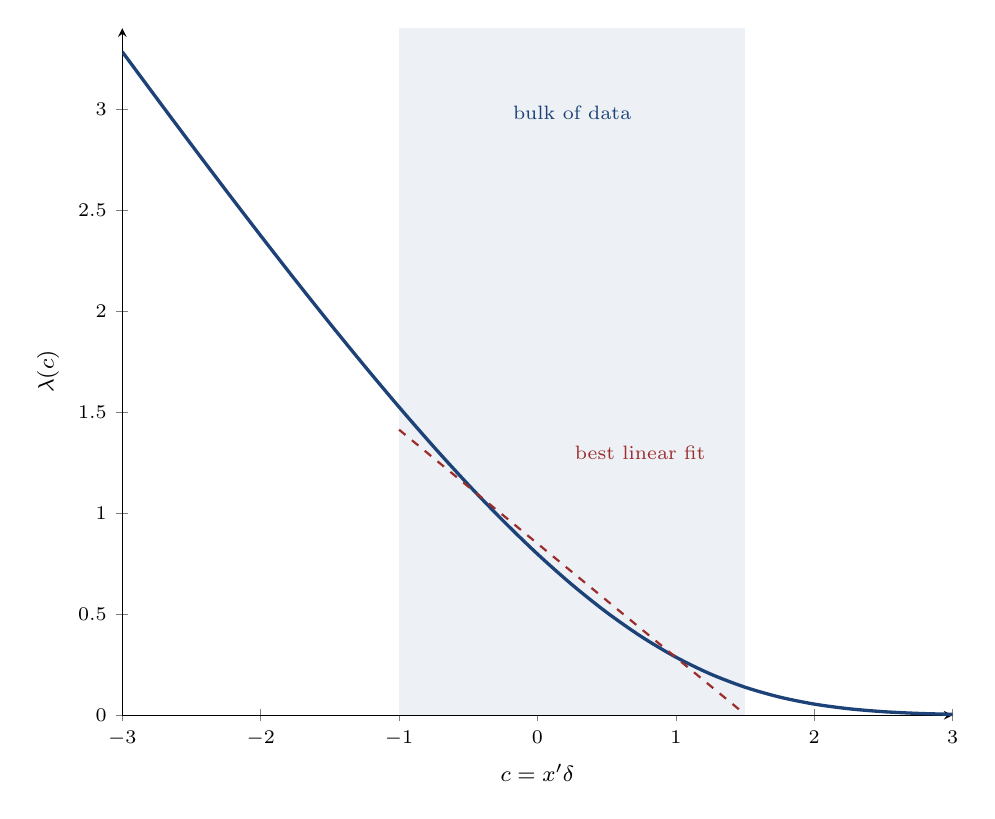
\begin{tikzpicture}
\begin{axis}[
  width=\linewidth, height=0.85\linewidth,
  xmin=-3, xmax=3, ymin=0, ymax=3.4,
  xlabel={$c=x'\delta$}, ylabel={$\Mills(c)$},
  xlabel style={font=\footnotesize}, ylabel style={font=\footnotesize},
  tick label style={font=\scriptsize},
  axis lines=left
]
\fill[DeepBlue!8] (axis cs:-1,0) rectangle (axis cs:1.5,3.4);
\addplot[DeepBlue, very thick, smooth] coordinates {
(-3.00,3.2831) (-2.75,3.0518) (-2.50,2.8227) (-2.25,2.5964) (-2.00,2.3732)
(-1.75,2.1537) (-1.50,1.9387) (-1.25,1.7288) (-1.00,1.5251) (-0.75,1.3288)
(-0.50,1.1411) (-0.25,0.9636) (0.00,0.7979) (0.25,0.6458) (0.50,0.5092)
(0.75,0.3894) (1.00,0.2876) (1.25,0.2042) (1.50,0.1388) (1.75,0.0899)
(2.00,0.0552) (2.25,0.0321) (2.50,0.0176) (2.75,0.0091) (3.00,0.0044)};
\addplot[DarkRed, thick, dashed, domain=-1:1.5] {0.8497-0.5634*x};
\node[font=\scriptsize, DarkRed, anchor=west] at (axis cs:0.2,1.3) {best linear fit};
\node[font=\scriptsize, DeepBlue, anchor=south] at (axis cs:0.25,2.9) {bulk of data};
\end{axis}
\end{tikzpicture}

\end{columns}

\end{frame}

% =========================================================
\begin{frame}{\Part{3} What is identified without leaning on normality?}

\begin{block}{Reduced-form objects that are always identified}
\begin{itemize}
  \item $\Pp(d=1\mid x)=\Phi(x'\delta)$, so $\delta$ \hfill (participation equation)
  \item $\E[y\mid x,d=1]$ \hfill (the wage regression \emph{among workers})
\end{itemize}
\end{block}

\pause

Drop normality and let the selection term be an unknown function $g$:
\[
\E[y\mid x,d=1]=x'\beta+g(x'\delta).
\]
For any constant $c$, the pair $\big(\beta+c\,\delta,\;g(t)-c\,t\big)$ fits the
data equally well:
\[
\boxed{\beta \text{ is identified only up to } \beta+c\,\delta}
\]
Only the part of $\beta$ not in the direction of $\delta$
(e.g.\ $\beta_k-\beta_1\delta_k/\delta_1$) is learned.

\pause

\begin{alertblock}{The parallel with Part I}
Part I without exclusion: only $\gamma+\rho/\sigma_w$ is identified.
Part II without exclusion: only $\beta$ modulo the direction $\delta$.
In both, the causal and the selection components cannot be separated.
\end{alertblock}

\end{frame}

% =========================================================
\subsection{(4) Stata}

\begin{frame}[fragile]{\Part{4} Stata}

Same \texttt{mroz} data: \texttt{lwage} $=y$, \texttt{inlf} $=d$; excluded:
\texttt{nwifeinc}, \texttt{age}, \texttt{kidslt6}, \texttt{kidsge6}.

\begin{lstlisting}[style=stata]
// (a) Full MLE (default): reports rho, sigma, lambda = rho*sigma, LR test of rho = 0
heckman lwage educ exper expersq, ///
        select(inlf = educ exper expersq nwifeinc age kidslt6 kidsge6)

// (b) Heckman two-step with corrected standard errors
heckman lwage educ exper expersq, ///
        select(inlf = educ exper expersq nwifeinc age kidslt6 kidsge6) twostep

// (c) By hand: point estimates only
probit  inlf educ exper expersq nwifeinc age kidslt6 kidsge6
predict zd, xb
generate mills = normalden(zd)/normal(zd)
regress lwage educ exper expersq mills if inlf == 1

// Postestimation after (a) or (b)
predict yhat,  xb        // E[y|x]: the wage offer
predict ycond, ycond     // E[y|x, d=1]: observed wages
\end{lstlisting}

\vspace{-0.2em}
\footnotesize
Related: \texttt{heckprobit} (binary outcome with selection),
\texttt{eregress \ldots, select()} (Stata 15+).

\end{frame}

% =========================================================
\section{Synthesis}

\begin{frame}{Two problems, one structure}

\small

\begin{tabular}{B{0.21\textwidth} L{0.34\textwidth} L{0.36\textwidth}}
\toprule
& Part I: endogenous probit & Part II: Heckman selection\\
\midrule
What is endogenous? & A regressor, $w$ & The sample, $d=1$\\[0.1em]
First stage & Linear regression of $w$ & Probit of $d$\\[0.1em]
Control function & $\rho\,v$ & $\rho\sigma\,\Mills(z'\delta)$\\[0.1em]
Second stage & Probit with $\hat v$ & OLS with $\hat\Mills$\\[0.1em]
Exclusion & $z\in x_w$, $z\notin x_y$ & $z$ in selection, not in $x$\\[0.1em]
Without exclusion & Exactly not identified; only $\gamma+\rho/\sigma_w$ &
  Only through the nonlinearity of $\Mills$\\[0.1em]
Free exogeneity test & $t$-test on $\hat v$ & $t$-test on $\hat\Mills$\\[0.1em]
Stata & \texttt{ivprobit} & \texttt{heckman}\\
\bottomrule
\end{tabular}

\vspace{0.1em}

\begin{block}{The common recipe}
\Spec: write down the joint normal model.
\Ident: condition on the first-stage residual, then find variation
that moves the endogenous object but not the outcome.
\Est: two-step or MLE.
\Infer: correct for generated regressors.
\end{block}

\end{frame}

% =========================================================
\begin{frame}{Takeaways}

\begin{enumerate}
  \item
  Under joint normality, endogeneity and selection both become
  \textbf{omitted-variable problems}, and the omitted variable is a
  control function: $v$ or $\Mills$.

  \vspace{0.25em}

  \item
  Identification comes from an \textbf{exclusion restriction}, not from
  the probit or the normal distribution.

  \vspace{0.25em}

  \item
  Without an exclusion restriction, Part I fails \emph{exactly}, while
  Part II hangs on the curvature of $\Mills$: a thread, not an
  identification strategy.

  \vspace{0.25em}

  \item
  Two-step estimators are easy and transparent but need corrected
  standard errors; MLE is efficient but leans harder on normality.

  \vspace{0.25em}

  \item
  The same variable can be endogenous in one question and an instrument
  in another.
\end{enumerate}

\end{frame}

% =========================================================
\begin{frame}{One sentence to remember}

\begin{center}

\vspace{0.6em}

\Huge
\textbf{
A control function
\\[0.3em]
is only as good as
\\[0.3em]
its excluded variable.
}

\end{center}

\end{frame}

% =========================================================
\begin{frame}{Selected references}

\scriptsize

Blundell, R., and J. L. Powell (2004).
``Endogeneity in Semiparametric Binary Response Models.''
\textit{Review of Economic Studies}, 71(3), 655--679.

\vspace{0.2em}

Gronau, R. (1974).
``Wage Comparisons---A Selectivity Bias.''
\textit{Journal of Political Economy}, 82(6), 1119--1143.

\vspace{0.2em}

Heckman, J. J. (1979).
``Sample Selection Bias as a Specification Error.''
\textit{Econometrica}, 47(1), 153--161.

\vspace{0.2em}

Lewbel, A. (2019).
``The Identification Zoo: Meanings of Identification in Econometrics.''
\textit{Journal of Economic Literature}, 57(4), 835--903.

\vspace{0.2em}

Mroz, T. A. (1987).
``The Sensitivity of an Empirical Model of Married Women's Hours of Work
to Economic and Statistical Assumptions.''
\textit{Econometrica}, 55(4), 765--799.

\vspace{0.2em}

Newey, W. K. (1987).
``Efficient Estimation of Limited Dependent Variable Models with
Endogenous Explanatory Variables.''
\textit{Journal of Econometrics}, 36(3), 231--250.

\vspace{0.2em}

Rivers, D., and Q. H. Vuong (1988).
``Limited Information Estimators and Exogeneity Tests for Simultaneous
Probit Models.''
\textit{Journal of Econometrics}, 39(3), 347--366.

\vspace{0.2em}

Smith, R. J., and R. W. Blundell (1986).
``An Exogeneity Test for a Simultaneous Equation Tobit Model with an
Application to Labor Supply.''
\textit{Econometrica}, 54(3), 679--685.

\vspace{0.2em}

Wooldridge, J. M. (2010).
\textit{Econometric Analysis of Cross Section and Panel Data}, 2nd ed.
MIT Press, Chapters 15 and 19.

\end{frame}

\end{document}
